\documentclass[twoside]{book}

% Packages required by doxygen
\usepackage{fixltx2e}
\usepackage{calc}
\usepackage{doxygen}
\usepackage[export]{adjustbox} % also loads graphicx
\usepackage{graphicx}
\usepackage[utf8]{inputenc}
\usepackage{makeidx}
\usepackage{multicol}
\usepackage{multirow}
\PassOptionsToPackage{warn}{textcomp}
\usepackage{textcomp}
\usepackage[nointegrals]{wasysym}
\usepackage[table]{xcolor}

% Font selection
\usepackage[T1]{fontenc}
\usepackage[scaled=.90]{helvet}
\usepackage{courier}
\usepackage{amssymb}
\usepackage{sectsty}
\renewcommand{\familydefault}{\sfdefault}
\allsectionsfont{%
  \fontseries{bc}\selectfont%
  \color{darkgray}%
}
\renewcommand{\DoxyLabelFont}{%
  \fontseries{bc}\selectfont%
  \color{darkgray}%
}
\newcommand{\+}{\discretionary{\mbox{\scriptsize$\hookleftarrow$}}{}{}}

% Page & text layout
\usepackage{geometry}
\geometry{%
  a4paper,%
  top=2.5cm,%
  bottom=2.5cm,%
  left=2.5cm,%
  right=2.5cm%
}
\tolerance=750
\hfuzz=15pt
\hbadness=750
\setlength{\emergencystretch}{15pt}
\setlength{\parindent}{0cm}
\setlength{\parskip}{3ex plus 2ex minus 2ex}
\makeatletter
\renewcommand{\paragraph}{%
  \@startsection{paragraph}{4}{0ex}{-1.0ex}{1.0ex}{%
    \normalfont\normalsize\bfseries\SS@parafont%
  }%
}
\renewcommand{\subparagraph}{%
  \@startsection{subparagraph}{5}{0ex}{-1.0ex}{1.0ex}{%
    \normalfont\normalsize\bfseries\SS@subparafont%
  }%
}
\makeatother

% Headers & footers
\usepackage{fancyhdr}
\pagestyle{fancyplain}
\fancyhead[LE]{\fancyplain{}{\bfseries\thepage}}
\fancyhead[CE]{\fancyplain{}{}}
\fancyhead[RE]{\fancyplain{}{\bfseries\leftmark}}
\fancyhead[LO]{\fancyplain{}{\bfseries\rightmark}}
\fancyhead[CO]{\fancyplain{}{}}
\fancyhead[RO]{\fancyplain{}{\bfseries\thepage}}
\fancyfoot[LE]{\fancyplain{}{}}
\fancyfoot[CE]{\fancyplain{}{}}
\fancyfoot[RE]{\fancyplain{}{\bfseries\scriptsize Generated by Doxygen }}
\fancyfoot[LO]{\fancyplain{}{\bfseries\scriptsize Generated by Doxygen }}
\fancyfoot[CO]{\fancyplain{}{}}
\fancyfoot[RO]{\fancyplain{}{}}
\renewcommand{\footrulewidth}{0.4pt}
\renewcommand{\chaptermark}[1]{%
  \markboth{#1}{}%
}
\renewcommand{\sectionmark}[1]{%
  \markright{\thesection\ #1}%
}

% Indices & bibliography
\usepackage{natbib}
\usepackage[titles]{tocloft}
\setcounter{tocdepth}{3}
\setcounter{secnumdepth}{5}
\makeindex

% Hyperlinks (required, but should be loaded last)
\usepackage{ifpdf}
\ifpdf
  \usepackage[pdftex,pagebackref=true]{hyperref}
\else
  \usepackage[ps2pdf,pagebackref=true]{hyperref}
\fi
\hypersetup{%
  colorlinks=true,%
  linkcolor=blue,%
  citecolor=blue,%
  unicode%
}

% Custom commands
\newcommand{\clearemptydoublepage}{%
  \newpage{\pagestyle{empty}\cleardoublepage}%
}

\usepackage{caption}
\captionsetup{labelsep=space,justification=centering,font={bf},singlelinecheck=off,skip=4pt,position=top}

%===== C O N T E N T S =====

\begin{document}

% Titlepage & ToC
\hypersetup{pageanchor=false,
             bookmarksnumbered=true,
             pdfencoding=unicode
            }
\pagenumbering{roman}
\begin{titlepage}
\vspace*{7cm}
\begin{center}%
{\Large Coordinate }\\
\vspace*{1cm}
{\large Generated by Doxygen 1.8.11}\\
\end{center}
\end{titlepage}
\clearemptydoublepage
\tableofcontents
\clearemptydoublepage
\pagenumbering{arabic}
\hypersetup{pageanchor=true}

%--- Begin generated contents ---
\chapter{Hierarchical Index}
\section{Class Hierarchy}
This inheritance list is sorted roughly, but not completely, alphabetically\+:\begin{DoxyCompactList}
\item \contentsline{section}{I\+Coordinate\+Axis}{\pageref{class_i_coordinate_axis}}{}
\begin{DoxyCompactList}
\item \contentsline{section}{Coordinate\+Axis}{\pageref{class_coordinate_axis}}{}
\end{DoxyCompactList}
\item Node\+Callback\begin{DoxyCompactList}
\item \contentsline{section}{Coordinate\+Updater}{\pageref{class_coordinate_updater}}{}
\end{DoxyCompactList}
\end{DoxyCompactList}

\chapter{Class Index}
\section{Class List}
Here are the classes, structs, unions and interfaces with brief descriptions\+:\begin{DoxyCompactList}
\item\contentsline{section}{\hyperlink{class_coordinate_axis}{Coordinate\+Axis} }{\pageref{class_coordinate_axis}}{}
\item\contentsline{section}{\hyperlink{class_coordinate_updater}{Coordinate\+Updater} }{\pageref{class_coordinate_updater}}{}
\item\contentsline{section}{\hyperlink{class_i_coordinate_axis}{I\+Coordinate\+Axis} \\*$<$一个叫\+I\+Coordinate\+Axis的接口类 成员函数分别是根据属性制作一个坐标系和获取X,Y或\+Z轴的方向.$>$ }{\pageref{class_i_coordinate_axis}}{}
\end{DoxyCompactList}

\chapter{Class Documentation}
\hypertarget{class_coordinate_axis}{}\section{Coordinate\+Axis Class Reference}
\label{class_coordinate_axis}\index{Coordinate\+Axis@{Coordinate\+Axis}}


{\ttfamily \#include $<$Coordinate\+Axis.\+h$>$}

Inheritance diagram for Coordinate\+Axis\+:\begin{figure}[H]
\begin{center}
\leavevmode
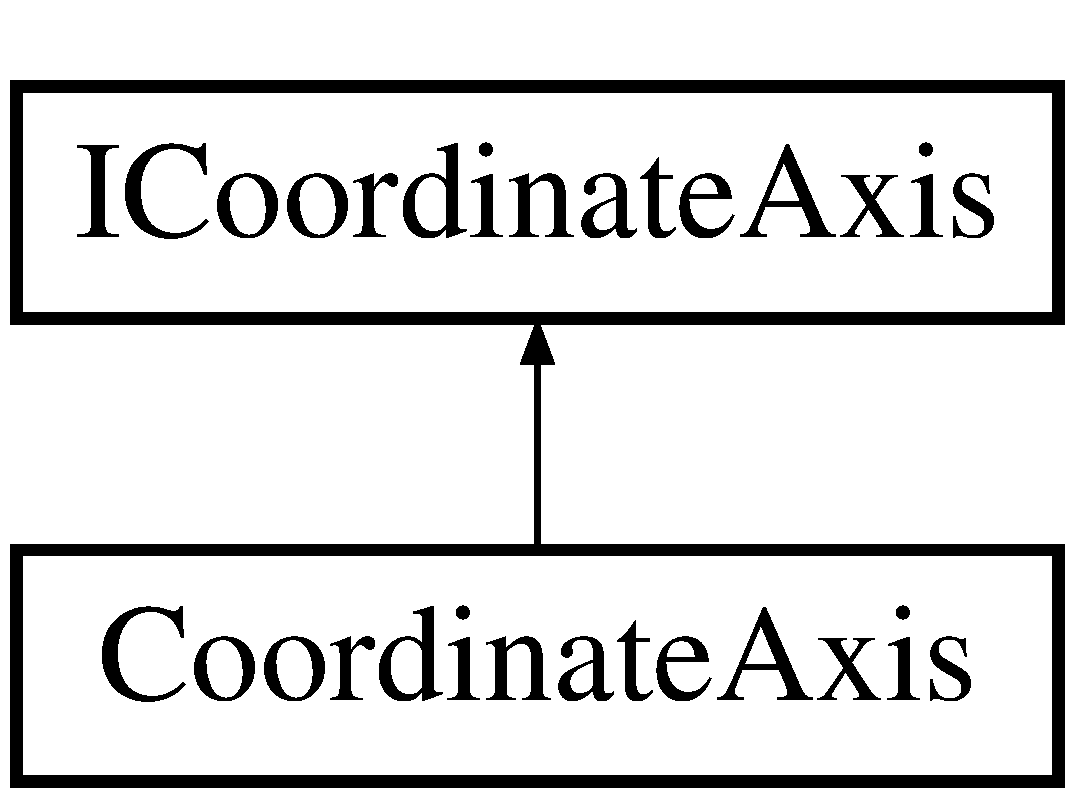
\includegraphics[height=2.000000cm]{class_coordinate_axis}
\end{center}
\end{figure}
\subsection*{Public Member Functions}
\begin{DoxyCompactItemize}
\item 
\hyperlink{class_coordinate_axis_a3dca3ab6abacbba77f64ef13e6184707}{Coordinate\+Axis} (osg\+G\+A\+::\+Multi\+Touch\+Trackball\+Manipulator $\ast$manip)
\begin{DoxyCompactList}\small\item\em $<$ 构造函数,对私有变量进行初始化$>$=\char`\"{}\char`\"{}$>$ \end{DoxyCompactList}\item 
\hyperlink{class_coordinate_axis_aeaf2a1f97ff54633e877b4b974839635}{$\sim$\+Coordinate\+Axis} ()\hypertarget{class_coordinate_axis_aeaf2a1f97ff54633e877b4b974839635}{}\label{class_coordinate_axis_aeaf2a1f97ff54633e877b4b974839635}

\begin{DoxyCompactList}\small\item\em 获取坐标轴方向$>$ \end{DoxyCompactList}\item 
virtual void \hyperlink{class_coordinate_axis_a97f2838c4ade40588c8e680f4ff51629}{get\+Axis\+Direction} (Axis ax, float \&x, float \&y, float \&z)
\begin{DoxyCompactList}\small\item\em 通过指定的二维屏幕坐标画出坐标系,可以指定坐标系的半径长度,需要把屏幕相机作为参数传进去$>$ \end{DoxyCompactList}\item 
virtual osg\+::\+Matrix\+Transform $\ast$ \hyperlink{class_coordinate_axis_acbd3e387e7cf1dd0d8ae83ed4073b5c2}{set\+Axis} (float x, float y, float radius, osg\+::\+Camera $\ast$camera)
\end{DoxyCompactItemize}


\subsection{Detailed Description}
class \hyperlink{class_coordinate_axis}{Coordinate\+Axis}

brief $<$ 继承于icoordinateaxis接口类,并对函数进行定义$>$=\char`\"{}\char`\"{}$>$

author Admin date 2016/3/14 

\subsection{Constructor \& Destructor Documentation}
\index{Coordinate\+Axis@{Coordinate\+Axis}!Coordinate\+Axis@{Coordinate\+Axis}}
\index{Coordinate\+Axis@{Coordinate\+Axis}!Coordinate\+Axis@{Coordinate\+Axis}}
\subsubsection[{\texorpdfstring{Coordinate\+Axis(osg\+G\+A\+::\+Multi\+Touch\+Trackball\+Manipulator $\ast$manip)}{CoordinateAxis(osgGA::MultiTouchTrackballManipulator *manip)}}]{\setlength{\rightskip}{0pt plus 5cm}Coordinate\+Axis\+::\+Coordinate\+Axis (
\begin{DoxyParamCaption}
\item[{osg\+G\+A\+::\+Multi\+Touch\+Trackball\+Manipulator $\ast$}]{manip}
\end{DoxyParamCaption}
)}\hypertarget{class_coordinate_axis_a3dca3ab6abacbba77f64ef13e6184707}{}\label{class_coordinate_axis_a3dca3ab6abacbba77f64ef13e6184707}


$<$ 构造函数,对私有变量进行初始化$>$=\char`\"{}\char`\"{}$>$ 

fn \hyperlink{class_coordinate_axis_a3dca3ab6abacbba77f64ef13e6184707}{Coordinate\+Axis\+::\+Coordinate\+Axis(osg\+G\+A\+::\+Multi\+Touch\+Trackball\+Manipulator$\ast$ manip)}

brief $<$ 构造函数,对私有变量的初始化$>$=\char`\"{}\char`\"{}$>$

author Admin date 2016/3/14

param \mbox{[}in,out\mbox{]} manip If non-\/null, the manip. 

\subsection{Member Function Documentation}
\index{Coordinate\+Axis@{Coordinate\+Axis}!get\+Axis\+Direction@{get\+Axis\+Direction}}
\index{get\+Axis\+Direction@{get\+Axis\+Direction}!Coordinate\+Axis@{Coordinate\+Axis}}
\subsubsection[{\texorpdfstring{get\+Axis\+Direction(\+Axis ax, float \&x, float \&y, float \&z)}{getAxisDirection(Axis ax, float &x, float &y, float &z)}}]{\setlength{\rightskip}{0pt plus 5cm}void Coordinate\+Axis\+::get\+Axis\+Direction (
\begin{DoxyParamCaption}
\item[{Axis}]{ax, }
\item[{float \&}]{x, }
\item[{float \&}]{y, }
\item[{float \&}]{z}
\end{DoxyParamCaption}
)\hspace{0.3cm}{\ttfamily [virtual]}}\hypertarget{class_coordinate_axis_a97f2838c4ade40588c8e680f4ff51629}{}\label{class_coordinate_axis_a97f2838c4ade40588c8e680f4ff51629}


通过指定的二维屏幕坐标画出坐标系,可以指定坐标系的半径长度,需要把屏幕相机作为参数传进去$>$ 

fn void \hyperlink{class_coordinate_axis_a97f2838c4ade40588c8e680f4ff51629}{Coordinate\+Axis\+::get\+Axis\+Direction(\+Axis ax, float \&x, float \&y, float \&z)}

brief $<$ 通过参数指定的轴向来获取向量$>$=\char`\"{}\char`\"{}$>$

author Admin date 2016/3/14

param ax The ax. param \mbox{[}out\mbox{]} x $<$指向的x向量.$>$ param \mbox{[}out\mbox{]} y $<$指向的y向量.$>$ param \mbox{[}out\mbox{]} z $<$指向的z向量.$>$ 

Implements \hyperlink{class_i_coordinate_axis_ad22ead68acd66ed2d191017fd12697b7}{I\+Coordinate\+Axis}.

\index{Coordinate\+Axis@{Coordinate\+Axis}!set\+Axis@{set\+Axis}}
\index{set\+Axis@{set\+Axis}!Coordinate\+Axis@{Coordinate\+Axis}}
\subsubsection[{\texorpdfstring{set\+Axis(float x, float y, float radius, osg\+::\+Camera $\ast$camera)}{setAxis(float x, float y, float radius, osg::Camera *camera)}}]{\setlength{\rightskip}{0pt plus 5cm}osg\+::\+Matrix\+Transform $\ast$ Coordinate\+Axis\+::set\+Axis (
\begin{DoxyParamCaption}
\item[{float}]{x, }
\item[{float}]{y, }
\item[{float}]{radius, }
\item[{osg\+::\+Camera $\ast$}]{camera}
\end{DoxyParamCaption}
)\hspace{0.3cm}{\ttfamily [virtual]}}\hypertarget{class_coordinate_axis_acbd3e387e7cf1dd0d8ae83ed4073b5c2}{}\label{class_coordinate_axis_acbd3e387e7cf1dd0d8ae83ed4073b5c2}
fn osg\+::\+Matrix\+Transform$\ast$ \hyperlink{class_coordinate_axis_acbd3e387e7cf1dd0d8ae83ed4073b5c2}{Coordinate\+Axis\+::set\+Axis(float x, float y, float radius, osg\+::\+Camera $\ast$camera)}

brief $<$通过指定的二维屏幕坐标画出坐标系,可以指定坐标系的半径长度,需要把屏幕相机作为参数传进去

author Admin date 2016/3/14

param x $<$屏幕的二维横坐标.$>$ param y $<$屏幕的二维纵坐标.$>$ param radius $<$坐标系 的边长.$>$ param \mbox{[}in\mbox{]} camera If non-\/null, the camera.

return null if it fails, else a pointer to an osg\+::\+Matrix\+Transform. 

Implements \hyperlink{class_i_coordinate_axis_a4e5694296507a4e86e0fdfbd4ba6a4b8}{I\+Coordinate\+Axis}.



The documentation for this class was generated from the following files\+:\begin{DoxyCompactItemize}
\item 
Coordinate\+Device/Coordinate\+Axis.\+h\item 
Coordinate\+Device/Coordinate\+Axis.\+cpp\end{DoxyCompactItemize}

\hypertarget{class_coordinate_updater}{}\section{Coordinate\+Updater Class Reference}
\label{class_coordinate_updater}\index{Coordinate\+Updater@{Coordinate\+Updater}}


{\ttfamily \#include $<$Coordinate\+Updater.\+h$>$}

Inheritance diagram for Coordinate\+Updater\+:\begin{figure}[H]
\begin{center}
\leavevmode
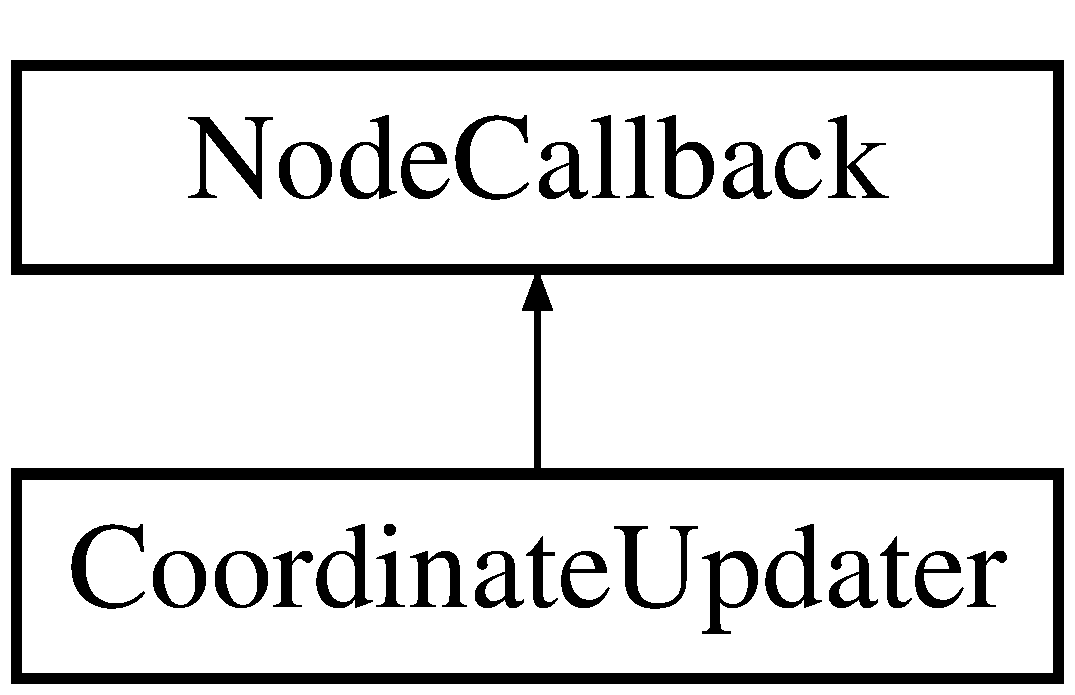
\includegraphics[height=2.000000cm]{class_coordinate_updater}
\end{center}
\end{figure}
\subsection*{Public Member Functions}
\begin{DoxyCompactItemize}
\item 
\hyperlink{class_coordinate_updater_afb57ab6d123b7c37fb22b98d212c6be9}{Coordinate\+Updater} (osg\+G\+A\+::\+Multi\+Touch\+Trackball\+Manipulator $\ast$manip)
\begin{DoxyCompactList}\small\item\em brief $<$ 构造私有成员进行初始化,利用传进来的manip来表示当前的环境$>$=\char`\"{}\char`\"{}$>$ \end{DoxyCompactList}\item 
virtual void \hyperlink{class_coordinate_updater_af67e8d382ffd471a058102d35cbd988c}{operator()} (osg\+::\+Node $\ast$node, osg\+::\+Node\+Visitor $\ast$nv) override
\begin{DoxyCompactList}\small\item\em $<$对传进来的manip进行操作.$>$ \end{DoxyCompactList}\item 
osg\+::\+Vec3 \hyperlink{class_coordinate_updater_ae9125c8a126d0e98b0dd6711b37f6876}{get\+Result} (Axis ax)
\begin{DoxyCompactList}\small\item\em $<$ 根据传进来\+Axis的枚举值,来确定获取哪个轴的结果.$>$ \end{DoxyCompactList}\end{DoxyCompactItemize}


\subsection{Detailed Description}
class \hyperlink{class_coordinate_updater}{Coordinate\+Updater}

brief $<$一个继承于osg\+::\+Node\+Callback的类,能够使处于\+H\+U\+D相机下的坐标系能够用鼠标控制旋转,并且能够计数刷新$>$

author Admin date 2016/3/14 

\subsection{Constructor \& Destructor Documentation}
\index{Coordinate\+Updater@{Coordinate\+Updater}!Coordinate\+Updater@{Coordinate\+Updater}}
\index{Coordinate\+Updater@{Coordinate\+Updater}!Coordinate\+Updater@{Coordinate\+Updater}}
\subsubsection[{\texorpdfstring{Coordinate\+Updater(osg\+G\+A\+::\+Multi\+Touch\+Trackball\+Manipulator $\ast$manip)}{CoordinateUpdater(osgGA::MultiTouchTrackballManipulator *manip)}}]{\setlength{\rightskip}{0pt plus 5cm}Coordinate\+Updater\+::\+Coordinate\+Updater (
\begin{DoxyParamCaption}
\item[{osg\+G\+A\+::\+Multi\+Touch\+Trackball\+Manipulator $\ast$}]{manip}
\end{DoxyParamCaption}
)}\hypertarget{class_coordinate_updater_afb57ab6d123b7c37fb22b98d212c6be9}{}\label{class_coordinate_updater_afb57ab6d123b7c37fb22b98d212c6be9}


brief $<$ 构造私有成员进行初始化,利用传进来的manip来表示当前的环境$>$=\char`\"{}\char`\"{}$>$ 

brief $<$ 构造私有成员进行初始化,利用传进来的manip来表示当前的环境$>$=\char`\"{}\char`\"{}$>$

author Admin date 2016/3/14

param \mbox{[}in\mbox{]} manip If non-\/null, the manip. 

\subsection{Member Function Documentation}
\index{Coordinate\+Updater@{Coordinate\+Updater}!get\+Result@{get\+Result}}
\index{get\+Result@{get\+Result}!Coordinate\+Updater@{Coordinate\+Updater}}
\subsubsection[{\texorpdfstring{get\+Result(\+Axis ax)}{getResult(Axis ax)}}]{\setlength{\rightskip}{0pt plus 5cm}osg\+::\+Vec3 Coordinate\+Updater\+::get\+Result (
\begin{DoxyParamCaption}
\item[{Axis}]{ax}
\end{DoxyParamCaption}
)}\hypertarget{class_coordinate_updater_ae9125c8a126d0e98b0dd6711b37f6876}{}\label{class_coordinate_updater_ae9125c8a126d0e98b0dd6711b37f6876}


$<$ 根据传进来\+Axis的枚举值,来确定获取哪个轴的结果.$>$ 

fn osg\+::\+Vec3 \hyperlink{class_coordinate_updater_ae9125c8a126d0e98b0dd6711b37f6876}{Coordinate\+Updater\+::get\+Result(\+Axis ax)}

brief $<$根据传进来\+Axis的枚举值,来确定获取哪个轴的结果.$>$

author Admin date 2016/3/14

param ax $<$Axis类型的枚举值,代表着X,Y,Z轴$>$

return The result. $<$x\+Axis(1,0,0)代表着\+X轴$>$

y\+Axis(0,1,0)代表着\+Y轴$>$

$<$z\+Axis(0,0,1)代表着\+Z轴$>$ \index{Coordinate\+Updater@{Coordinate\+Updater}!operator()@{operator()}}
\index{operator()@{operator()}!Coordinate\+Updater@{Coordinate\+Updater}}
\subsubsection[{\texorpdfstring{operator()(osg\+::\+Node $\ast$node, osg\+::\+Node\+Visitor $\ast$nv) override}{operator()(osg::Node *node, osg::NodeVisitor *nv) override}}]{\setlength{\rightskip}{0pt plus 5cm}void Coordinate\+Updater\+::operator() (
\begin{DoxyParamCaption}
\item[{osg\+::\+Node $\ast$}]{node, }
\item[{osg\+::\+Node\+Visitor $\ast$}]{nv}
\end{DoxyParamCaption}
)\hspace{0.3cm}{\ttfamily [override]}, {\ttfamily [virtual]}}\hypertarget{class_coordinate_updater_af67e8d382ffd471a058102d35cbd988c}{}\label{class_coordinate_updater_af67e8d382ffd471a058102d35cbd988c}


$<$对传进来的manip进行操作.$>$ 

fn void \hyperlink{class_coordinate_updater_af67e8d382ffd471a058102d35cbd988c}{Coordinate\+Updater\+::operator()(osg\+::\+Node$\ast$ node, osg\+::\+Node\+Visitor$\ast$ nv)}

brief $<$对传进来的manip进行操作.\+让处于\+H\+U\+D相机的坐标系能够进行操作$>$

author Admin date 2016/3/14

param \mbox{[}in\mbox{]} $<$ 基类函数定义不需要管$>$=\char`\"{}\char`\"{}$>$ param \mbox{[}in\mbox{]} $<$基类函数定义不需要管.$>$ 

The documentation for this class was generated from the following files\+:\begin{DoxyCompactItemize}
\item 
Coordinate\+Device/Coordinate\+Updater.\+h\item 
Coordinate\+Device/Coordinate\+Update.\+cpp\end{DoxyCompactItemize}

\hypertarget{class_i_coordinate_axis}{}\section{I\+Coordinate\+Axis Class Reference}
\label{class_i_coordinate_axis}\index{I\+Coordinate\+Axis@{I\+Coordinate\+Axis}}


$<$一个叫\+I\+Coordinate\+Axis的接口类 成员函数分别是根据属性制作一个坐标系和获取X,Y或\+Z轴的方向.$>$  




{\ttfamily \#include $<$I\+Coordinate\+Axis.\+h$>$}

Inheritance diagram for I\+Coordinate\+Axis\+:\begin{figure}[H]
\begin{center}
\leavevmode
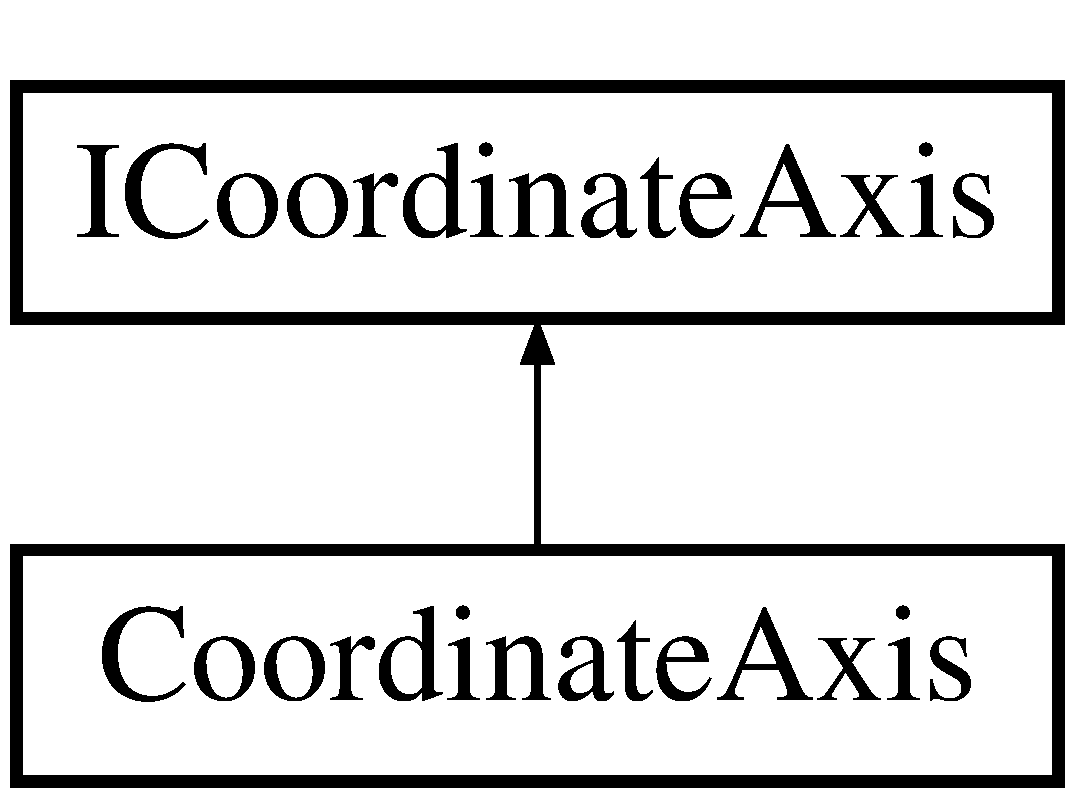
\includegraphics[height=2.000000cm]{class_i_coordinate_axis}
\end{center}
\end{figure}
\subsection*{Public Member Functions}
\begin{DoxyCompactItemize}
\item 
virtual void \hyperlink{class_i_coordinate_axis_ad22ead68acd66ed2d191017fd12697b7}{get\+Axis\+Direction} (Axis ax, float \&x, float \&y, float \&z)=0
\begin{DoxyCompactList}\small\item\em $<$获取某一个轴的指向.$>$ \end{DoxyCompactList}\item 
virtual osg\+::\+Matrix\+Transform $\ast$ \hyperlink{class_i_coordinate_axis_a4e5694296507a4e86e0fdfbd4ba6a4b8}{set\+Axis} (float x, float y, float radius, osg\+::\+Camera $\ast$camera)=0
\begin{DoxyCompactList}\small\item\em $<$ 通过指定的二维屏幕坐标画出坐标系,可以指定坐标系的半径长度,需要把屏幕相机作为参数传进去$>$=\char`\"{}\char`\"{}$>$ \end{DoxyCompactList}\end{DoxyCompactItemize}


\subsection{Detailed Description}
$<$一个叫\+I\+Coordinate\+Axis的接口类 成员函数分别是根据属性制作一个坐标系和获取X,Y或\+Z轴的方向.$>$ 

\begin{DoxyAuthor}{Author}
Admin 
\end{DoxyAuthor}
\begin{DoxyDate}{Date}
2016/3/14 
\end{DoxyDate}


\subsection{Member Function Documentation}
\index{I\+Coordinate\+Axis@{I\+Coordinate\+Axis}!get\+Axis\+Direction@{get\+Axis\+Direction}}
\index{get\+Axis\+Direction@{get\+Axis\+Direction}!I\+Coordinate\+Axis@{I\+Coordinate\+Axis}}
\subsubsection[{\texorpdfstring{get\+Axis\+Direction(\+Axis ax, float \&x, float \&y, float \&z)=0}{getAxisDirection(Axis ax, float &x, float &y, float &z)=0}}]{\setlength{\rightskip}{0pt plus 5cm}void I\+Coordinate\+Axis\+::get\+Axis\+Direction (
\begin{DoxyParamCaption}
\item[{Axis}]{ax, }
\item[{float \&}]{x, }
\item[{float \&}]{y, }
\item[{float \&}]{z}
\end{DoxyParamCaption}
)\hspace{0.3cm}{\ttfamily [pure virtual]}}\hypertarget{class_i_coordinate_axis_ad22ead68acd66ed2d191017fd12697b7}{}\label{class_i_coordinate_axis_ad22ead68acd66ed2d191017fd12697b7}


$<$获取某一个轴的指向.$>$ 

$<$其中参数\+Axis代表着X,Y,Z这三个轴.$>$ $<$用了三个引用\&X,\&Y,\&Z,代表指向的向量.$>$

\begin{DoxyAuthor}{Author}
Admin 
\end{DoxyAuthor}
\begin{DoxyDate}{Date}
2016/3/14
\end{DoxyDate}

\begin{DoxyParams}[1]{Parameters}
 & {\em ax} & The ax. \\
\hline
\mbox{\tt out}  & {\em x} & $<$ 指向的x向量$>$=\char`\"{}\char`\"{}$>$ \\
\hline
\mbox{\tt out}  & {\em y} & $<$ 指向的y向量$>$=\char`\"{}\char`\"{}$>$ \\
\hline
\mbox{\tt out}  & {\em z} & $<$ 指向的z向量$>$=\char`\"{}\char`\"{}$>$ \\
\hline
\end{DoxyParams}


Implemented in \hyperlink{class_coordinate_axis_a97f2838c4ade40588c8e680f4ff51629}{Coordinate\+Axis}.

\index{I\+Coordinate\+Axis@{I\+Coordinate\+Axis}!set\+Axis@{set\+Axis}}
\index{set\+Axis@{set\+Axis}!I\+Coordinate\+Axis@{I\+Coordinate\+Axis}}
\subsubsection[{\texorpdfstring{set\+Axis(float x, float y, float radius, osg\+::\+Camera $\ast$camera)=0}{setAxis(float x, float y, float radius, osg::Camera *camera)=0}}]{\setlength{\rightskip}{0pt plus 5cm}osg\+::\+Matrix\+Transform $\ast$ I\+Coordinate\+Axis\+::set\+Axis (
\begin{DoxyParamCaption}
\item[{float}]{x, }
\item[{float}]{y, }
\item[{float}]{radius, }
\item[{osg\+::\+Camera $\ast$}]{camera}
\end{DoxyParamCaption}
)\hspace{0.3cm}{\ttfamily [pure virtual]}}\hypertarget{class_i_coordinate_axis_a4e5694296507a4e86e0fdfbd4ba6a4b8}{}\label{class_i_coordinate_axis_a4e5694296507a4e86e0fdfbd4ba6a4b8}


$<$ 通过指定的二维屏幕坐标画出坐标系,可以指定坐标系的半径长度,需要把屏幕相机作为参数传进去$>$=\char`\"{}\char`\"{}$>$ 

\begin{DoxyAuthor}{Author}
Admin 
\end{DoxyAuthor}
\begin{DoxyDate}{Date}
2016/3/14
\end{DoxyDate}

\begin{DoxyParams}[1]{Parameters}
 & {\em x} & $<$ 二维横坐标$>$=\char`\"{}\char`\"{}$>$ \\
\hline
 & {\em y} & $<$ 二维纵坐标$>$=\char`\"{}\char`\"{}$>$ \\
\hline
 & {\em radius} & $<$ 坐标轴边半径$>$=\char`\"{}\char`\"{}$>$ \\
\hline
\mbox{\tt in}  & {\em camera} & $<$ 把屏幕相机作为参数传进来$>$=\char`\"{}\char`\"{}$>$\\
\hline
\end{DoxyParams}
\begin{DoxyReturn}{Returns}
null if it fails, else a pointer to an osg\+::\+Matrix\+Transform. 
\end{DoxyReturn}


Implemented in \hyperlink{class_coordinate_axis_acbd3e387e7cf1dd0d8ae83ed4073b5c2}{Coordinate\+Axis}.



The documentation for this class was generated from the following file\+:\begin{DoxyCompactItemize}
\item 
Coordinate\+Device/I\+Coordinate\+Axis.\+h\end{DoxyCompactItemize}

%--- End generated contents ---

% Index
\backmatter
\newpage
\phantomsection
\clearemptydoublepage
\addcontentsline{toc}{chapter}{Index}
\printindex

\end{document}
